\subsection{Evaluation}
\label{sec:exp:eval}

\begin{table*}[t]
\centering
\caption{Comparison of methods on LOCOMO.}
\small
% \renewcommand{\arraystretch}{0.85} % 1.5 倍默认行高
\begin{tabular}{l|r|r|r|r|r|r|r|r|r|r}
\toprule
\multirow{2}{*}{Method} & \multicolumn{2}{c|}{Single-Hop}  & \multicolumn{2}{c|}{Multi-Hop} & \multicolumn{2}{c|}{Temporal}  & \multicolumn{2}{c|}{Open-Domain} & \multicolumn{2}{c}{Overall}\\ \cline{2-11}
 & F1 &  BLEU-1 & F1  & BLEU-1  & F1 & BLEU-1 & F1 & BLEU-1 & F1 & BLEU-1\\ \midrule
\multicolumn{11}{c}{Qwen2.5-7B-Instruct}\\ \midrule
{\tt A-MEM} &33.11& 27.59& 25.38& 18.36& 14.69& 12.19& 14.69& 12.55 & 26.71 & 21.75 \\ 
{\tt MemoryBank}  & 15.34&11.92 & 16.63& 12.41& 11.57&9.49 &16.09 & 11.16 & 14.84 & 11.46 \\ 
{\tt MemGPT} &21.31 & 16.57& 18.92& 13.64& 17.37& 13.61& 11.14& 8.06 & 19.42 & 15.51 \\ 
{\tt Mem0} & 25.92& 21.47& 19.43& 14.76&\snd{37.49} &\snd{31.26} & 16.93& 10.58 & 26.58 & 21.60 \\ 
{\tt Mem0\(^g\)} &27.90 &23.45 &21.14 & 13.98&35.70 & 30.54&18.67 & 13.44 & 27.71 & 22.57 \\ 
{\tt MemoChat} & 7.21 & 5.84 & 9.74 & 6.59 & 5.33 & 4.26 & 14.31 & 10.81 & 7.72 & 5.96 \\ 
{\tt Zep} & \fst{40.42} & \fst{34.59} & \snd{30.97} & \snd{20.31} & 22.64 & 17.82 & 21.79 & \fst{17.57} & \snd{33.82} & \snd{27.42} \\ 
{\tt MemTree} & 33.36 & 27.91 & 26.40 & 17.59 & 25.62 & 21.45 & 20.67 & 16.23 & 29.68 & 23.95 \\ 
{\tt MemoryOS} & 33.14 & 28.33 & 28.52 & 19.90 & 17.65 & 14.09 & \snd{22.05} & \snd{16.95} & 28.34 & 23.11 \\ 
{\tt MemOS} & \snd{39.55} & \snd{33.58} & \fst{34.04} & \fst{23.38} & \fst{37.55} & \fst{31.90} & \fst{22.55} & 16.51 & \fst{37.05} & \fst{30.30} \\
% {\tt Ours} & 45.11 & 38.87 & 30.01 & 21.66 & 32.23 & 26.92 & 18.92 & 14.88 & 38.03 & 31.73 \\ 
\midrule
\multicolumn{11}{c}{Qwen2.5-72B-Instruct}\\ \midrule
{\tt A-MEM} & 42.24& \fst{38.68}&27.87 & 21.97& 28.01& 22.64& \snd{23.27}& \fst{18.55}& 30.35& 25.46\\ 
{\tt MemoryBank} & 24.54& 20.26& 23.28& 18.62& 13.21& 10.18& 19.12& 14.35& 21.61 & 17.50\\  
{\tt MemGPT} & 28.78 & 21.15 & 24.21& 19.11&20.28 &16.37 & 16.42&13.42 & 25.40 & 20.30\\ 
{\tt Mem0} & 32.83 & 27.89 & 25.35 & 21.14&40.76 & 36.03& 21.04& 14.09& 32.38 & 27.51\\  
{\tt Mem0\(^g\)} & 29.58& 25.19 & 30.22 & 24.67& \snd{43.89}& \snd{38.44} & 20.37& 12.81& 32.07& 27.06\\  
{\tt MemoChat} & 12.79 & 10.02 & 13.16 & 9.19 & 16.64 & 13.91 & 15.43 & 11.65 &13.83 &10.78 \\ 
{\tt Zep} & 42.46 & 35.99 & 33.11 & 23.39 & 34.58 & 27.89 & 15.87 & 11.47 &37.45 &30.46 \\ 
{\tt MemTree} & 38.73 & 32.42 & 33.01 & 25.07 & 29.81 & 24.48 & 23.02 & 17.46 &34.85 &28.49 \\ 
{\tt MemoryOS} & \snd{43.56} & \snd{37.00} & \snd{36.32} & \fst{27.91} & 37.36 & 29.58 & 22.57 & \snd{18.22} &\snd{39.63} &\snd{32.62} \\ 
{\tt MemOS} & \fst{44.30} & 36.85 & \fst{36.67} & \snd{26.95} & \fst{49.59} & \fst{43.13} & \fst{24.88} & 17.87 & \fst{42.79}& \fst{35.16}\\
% {\tt Ours} & 48.01 & 41.78 & 38.08 & 29.32 & 43.97 & 37.63 & 24.27 & 20.31 & 43.87& 37.30\\
\bottomrule
% 11 & - & - & - & - & - & - & - & - & - & - & - & - & - \\ \hline
\end{tabular}
\label{tab:loco}
\end{table*}




\begin{tikzpicture}
\filldraw (0,0) -- (-0.15,0.08) -- (-0.15,-0.08) -- cycle ; 
\end{tikzpicture} \textbf{Exp.1. Overall performance.}
We first report the performance of all agent memory methods on both benchmarks across two model scales (Qwen2.5-7B-Instruct and Qwen2.5-72B-Instruct). Results on LONGMEMEVAL and LOCOMO are shown in Table~\ref{tab:lme} and Table~ \ref{tab:loco}, respectively. Based on these results, we draw the following observations:

(1) Tree-based memory methods (e.g., {\tt MemTree} and {\tt MemOS}) generally achieve strong performance by organizing memory in a multi-layered, multi-granularity fashion. Specifically, {\tt MemTree} attains the highest F1 score of 36.92 on LONGMEMEVAL at the 7B scale, while {\tt MemOS} achieves the highest F1 scores of 37.05 and 42.79 on LOCOMO at the 7B and 72B scales, respectively. Tree structures provide high-level conceptual summaries at upper layers while preserving fine-grained details at leaf nodes. A similar advantage can be realized through well-designed hierarchical architectures that facilitate efficient information flow and transformation across different levels of abstraction, as evidenced by the highly competitive results of {\tt MemoryOS} and {\tt Zep}.

% (1) Generally, tree-based memory methods (e.g., {\tt MemTree} and {\tt MemOS}) exhibit notable performance by naturally organizing memory information in a multi-layered, multi-granularity fashion. Specifically, {\tt MemTree} achieves the highest F1 score of 36.92 on LONGMEMEVAL, while {\tt MemOS} attains the highest F1 scores of 37.05 and 42.79 on LOCOMO across 7B and 72B scales, respectively. Tree structures provide high-level conceptual summaries at the top layers while preserving fine-grained details at the leaf nodes. This can also be achieved through well-designed hierarchical architectures, which facilitate efficient information flow and transformation across different layers of abstraction, such as the highly competitive results delivered by {\tt MemoryOS} and {\tt Zep}.

% (2) Maintaining information completeness is crucial for memory persistence, specifically regarding the archival of raw messages during the information extraction phase and the integration of original conversations for final response generation. For example, methods solely extracting graph-based triples may suffer from information loss compared to those preserving raw dialogue fragments, which may explain why {\tt Mem0} outperforms {\tt Mem0$^g$} in many cases.

(2) Preserving information completeness is crucial for effective memory persistence---specifically, retaining raw messages during the information extraction phase and incorporating original conversations during final response generation. For example, methods that exclusively extract graph-based triples may suffer from information loss compared to those that preserve raw dialogue fragments, which may explain why {\tt Mem0} outperforms {\tt Mem0$^g$} in many cases.


% (3)Effective memory organization requires mechanisms to build explicit or implicit connections between related information to enhance the coherence of the stored memories, which is particularly important for multi-hop reasoning tasks. Methods lacking such associative operations, such as {\tt MemoryBank}, {\tt MemGPT}, and {\tt MemoChat}, perform poorly on Multi-Session tasks of LONGMEMEVAL and Multi Hop tasks of LOCOMO. In contrast, although {\tt Mem0} does not feature an explicit 'connecting' operator, its strategy of concurrently updating similar memories during ingestion achieves a comparable integration effect.  Notably, on the Multi-Session tasks of LONGMEMEVAL, {\tt Mem0} achieves 18.60\% F1 and 26.19\% BLEU-1 improvements over {\tt MemoryBank}.
(3) Effective memory organization requires mechanisms that build explicit or implicit connections among related pieces of information, thereby enhancing the coherence of stored memories. This is particularly important for multi-hop reasoning tasks. Methods lacking such associative operations, such as {\tt MemoryBank}, {\tt MemGPT}, and {\tt MemoChat}, perform poorly on the Multi-Session tasks of LONGMEMEVAL and the Multi-Hop tasks of LOCOMO. In contrast, although {\tt Mem0} does not feature an explicit ``connecting'' operator, its strategy of concurrently updating similar memories during ingestion achieves a comparable integration effect. Notably, on the Multi-Session tasks of LONGMEMEVAL, {\tt Mem0} achieves 18.60\% F1 and 26.19\% BLEU-1 improvements over {\tt MemoryBank}.


% (4) Due to the complexity and the inherent difficulty of temporal reasoning, these tasks remains highly sensitive to the reasoning capacity of the backbone model. For instance, {\tt MemoryOS} and {\tt MemoChat} exhibit a performance leap of over $2\times$ as the backbone LLM scaled from 7B to 72B. To reduce this heavy dependency on LLM reasoning and improve system robustness, it is essential to design specialized architectural components for processing temporal information rather than relying purely on the model's in-context reasoning during final response generation.
(4) Due to the complexity and inherent difficulty of temporal reasoning, these tasks remain highly sensitive to the reasoning capacity of the backbone model. For instance, {\tt MemoryOS} and {\tt MemoChat} exhibit a performance leap exceeding $2\times$ on LOCOMO as the backbone LLM scales from 7B to 72B. To mitigate this heavy dependence on LLM reasoning and improve system robustness, it is essential to design specialized architectural components for temporal information processing rather than relying solely on the model's in-context reasoning during response generation.



% \begin{figure}[]
%     \centering
%     \setlength{\abovecaptionskip}{0.1cm}
%     % \setlength{\belowcaptionskip}{-0.05cm}
%     \ref{tokenleg} \\ [0.1cm]
% \begin{tikzpicture}[scale=0.50]
%     \begin{axis}[
%         legend style = {
%                     legend columns=5,
%                     inner sep=0pt,
%                     draw=none,
%                     font=\small\ttfamily,
%                     legend image post style={
%                         scale=0.7,
%                         line width=1pt,
%                         mark options={
%                             scale=1.4,
%                             line width=1pt,
%                         },
%                     },
%                 },
%         legend to name=tokenleg,
%         xmin=0.4, xmax=10.6,
%         ymin=0, ymax=8000,
%         % ymode=log,
%         major tick style = {line width=1.2pt},
%         minor tick style = {line width=1pt},
%         xtick = {1,4,7,10},
%         minor xtick = {2,3,5,6,8,9},
%         xticklabels = {1,4,7,10},
%         ytick = {0, 500, 1000, 1500, 2000, 5000, 6000, 7000, 8000},
%         yticklabels = {0, 500, 1000, 1500, 2000, 5000, 6000, 7000, 8000},
%         xticklabel style={font=\Huge}, 
%         yticklabel style={font=\Huge},
%         ylabel = \textbf{Average Token Costs},
%         ylabel style={font=\Huge},
%         xlabel = \textbf{Sessions},
%         xlabel style={font=\Huge},
%         mark size=6pt, 
%         width=0.8\textwidth,
%         height=0.6\textwidth,
%         % ticklabel style={font=\Huge},
%         every axis plot/.append style={line width = 2pt},
%         every axis/.append style={line width = 2pt},
%     ]
%     \addplot[w0, mark=o] table[x=token, y=A-MEM] {\locotoken};
%     \addplot[w1, mark=x] table[x=token, y=MemoryBank] {\locotoken};
%     \addplot[w2, mark=+] table[x=token, y=MemGPT] {\locotoken};
%     \addplot[w3, mark=square] table[x=token, y=Mem0] {\locotoken};
%     \addplot[w4, mark=triangle] table[x=token, y=Mem0$^g$] {\locotoken};
%     \addplot[w5, mark=diamond] table[x=token, y=MemoChat] {\locotoken};
%     \addplot[w6, mark=star] table[x=token, y=Zep] {\locotoken};
%     \addplot[w7, mark=asterisk] table[x=token, y=MemTree] {\locotoken};
%     \addplot[w8, mark=triangle, mark options={rotate=180}, 
%         legend image code/.code={
%             \draw[w8, mark options={rotate=180, scale=1.4}, mark indices={2}] plot coordinates {(0cm,0cm) (0.3cm,0cm) (0.6cm,0cm)};
%         }
%     ] table[x=token, y=MemoryOS] {\locotoken};
%     \addplot[w9, mark=triangle, mark options={rotate=270},
%         legend image code/.code={
%             \draw[w9, mark options={rotate=270, scale=1.4}, mark indices={2}] plot coordinates {(0cm,0cm) (0.3cm,0cm) (0.6cm,0cm)};
%         }
%     ] table[x=token, y=MemOS] {\locotoken};
%     \legend{A-MEM, MemoryBank, MemGPT, Mem0, Mem0$^g$, MemoChat, Zep, MemTree, MemoryOS, MemOS}
%     \end{axis}
% \end{tikzpicture}
% \caption{Average token costs per dialogue across sessions on LOCOMO.}
% \label{fig:token}
% \end{figure}


\begin{figure}[]
    \centering
    \setlength{\abovecaptionskip}{0cm}
    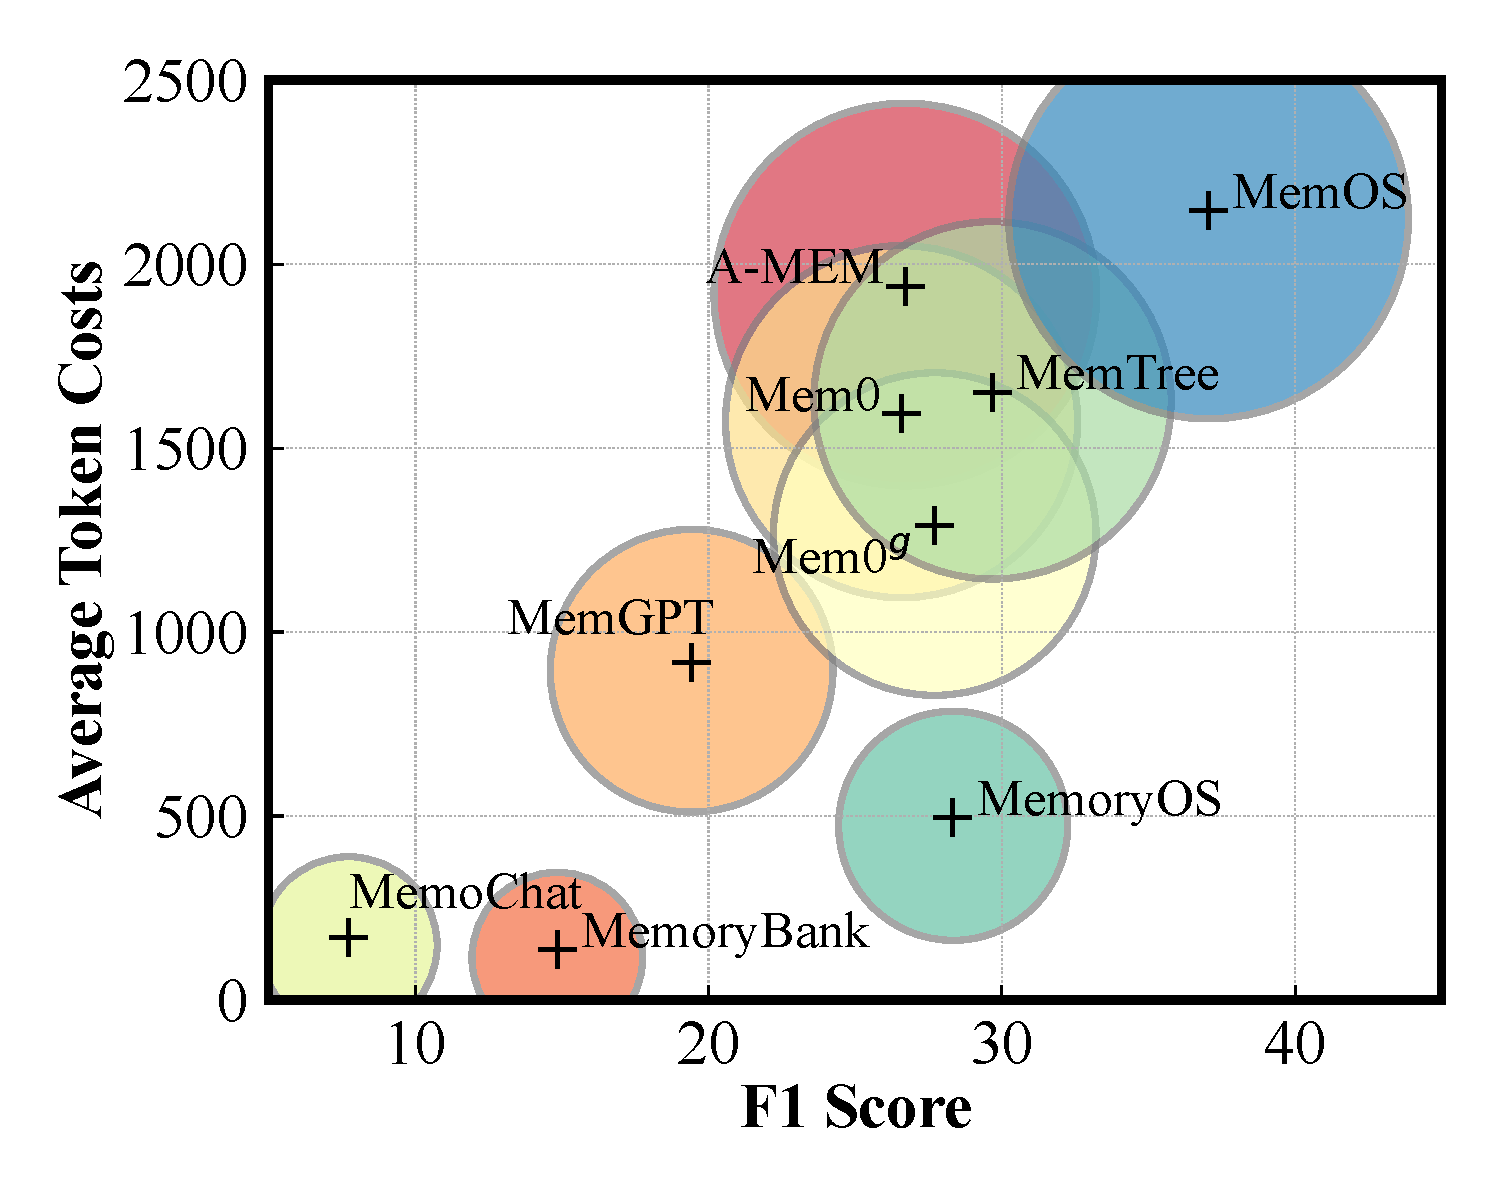
\includegraphics[width=0.87\linewidth]{figures/tradeoff.pdf}
    \caption{Overall trade-off between performance and token costs on LOCOMO.}
    \label{fig:tradeoff}
\end{figure}

\begin{figure}[]
    \centering
    \setlength{\abovecaptionskip}{0cm}
    \setlength{\belowcaptionskip}{-0.3cm}
    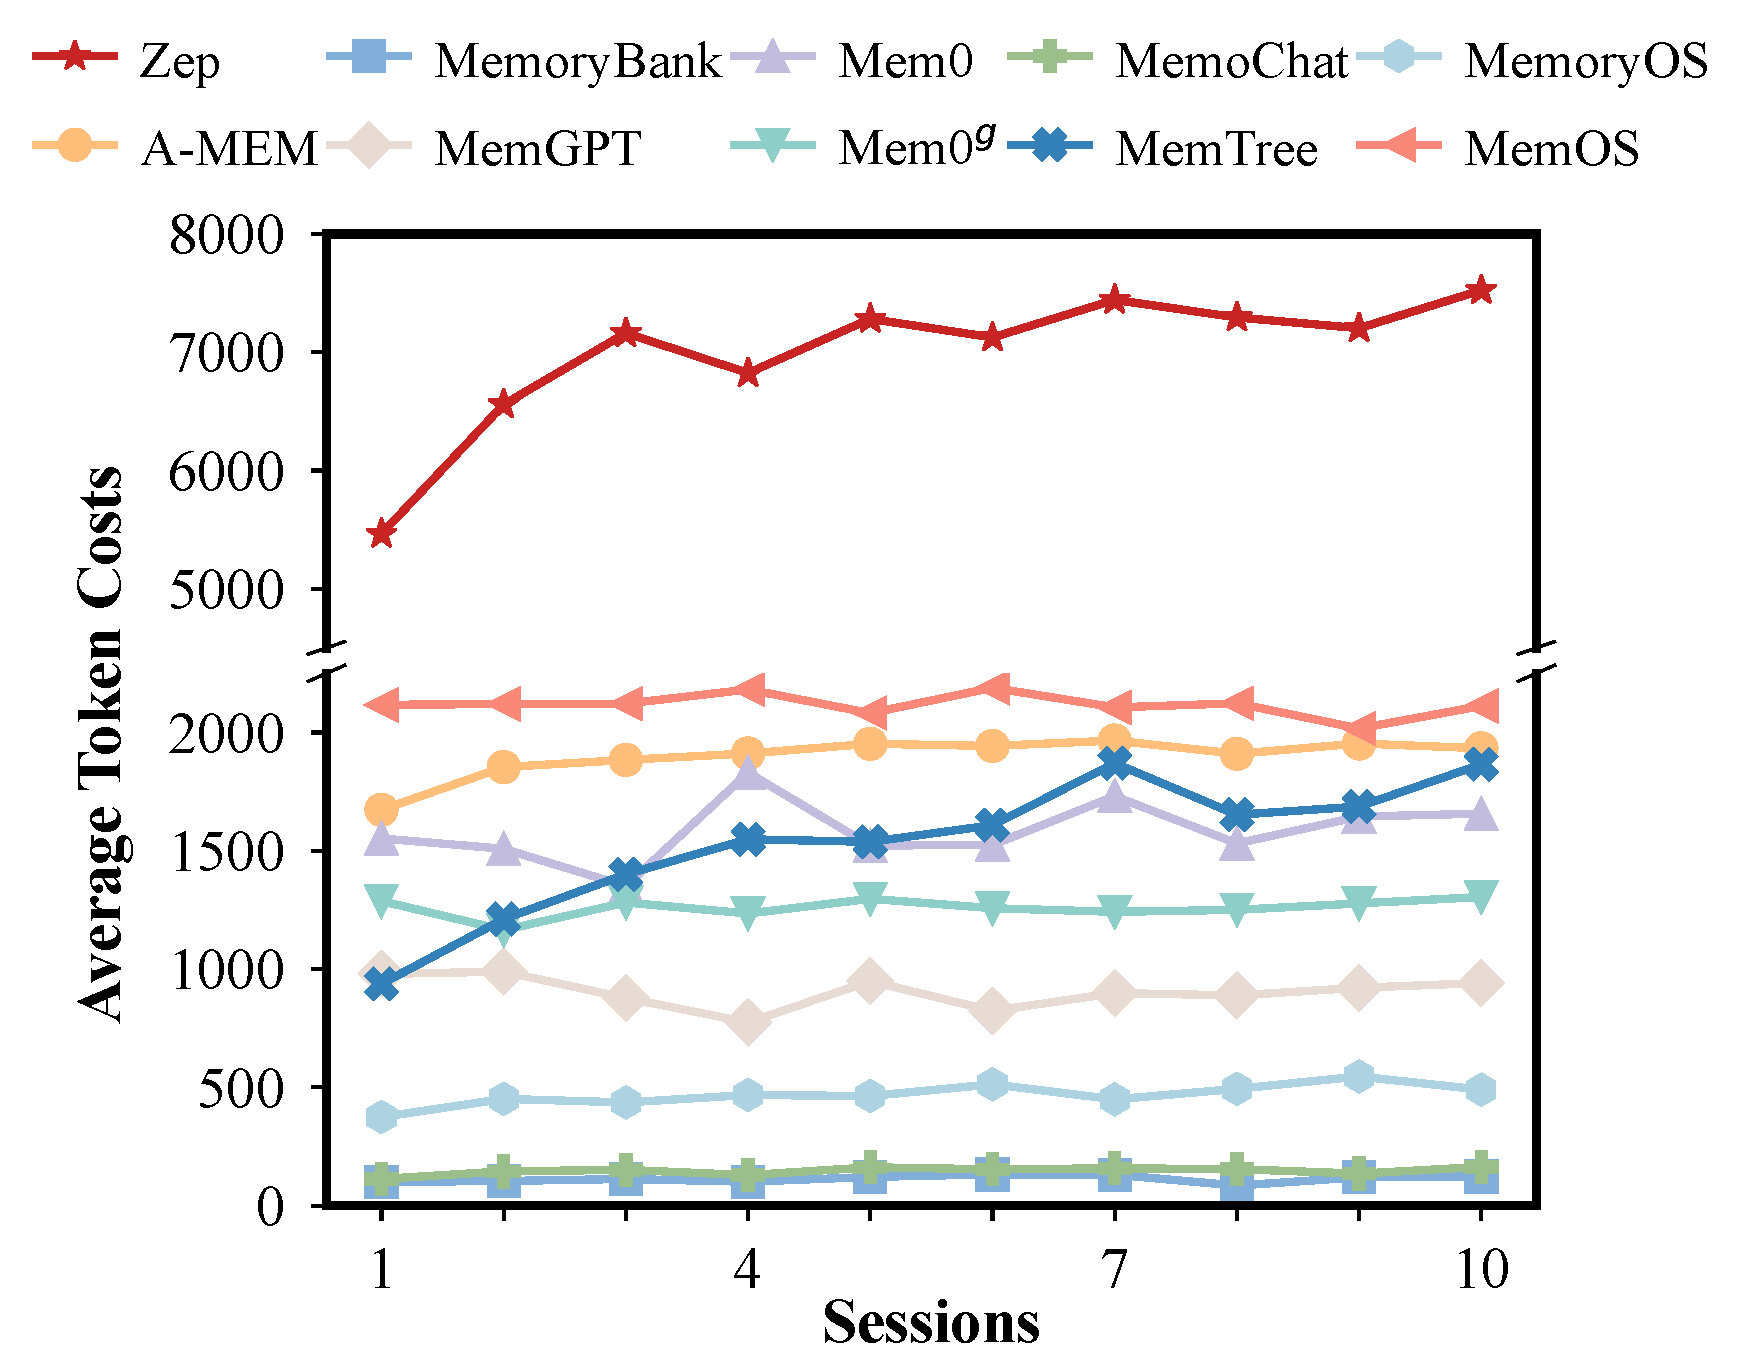
\includegraphics[width=\linewidth]{figures/token.pdf}
    \caption{Average token costs per dialogue across sessions on LOCOMO.}
    \label{fig:token}
\end{figure}

\begin{figure*}[t]
    \centering
    
    \begin{subfigure}[]{0.85\linewidth}
        \centering
        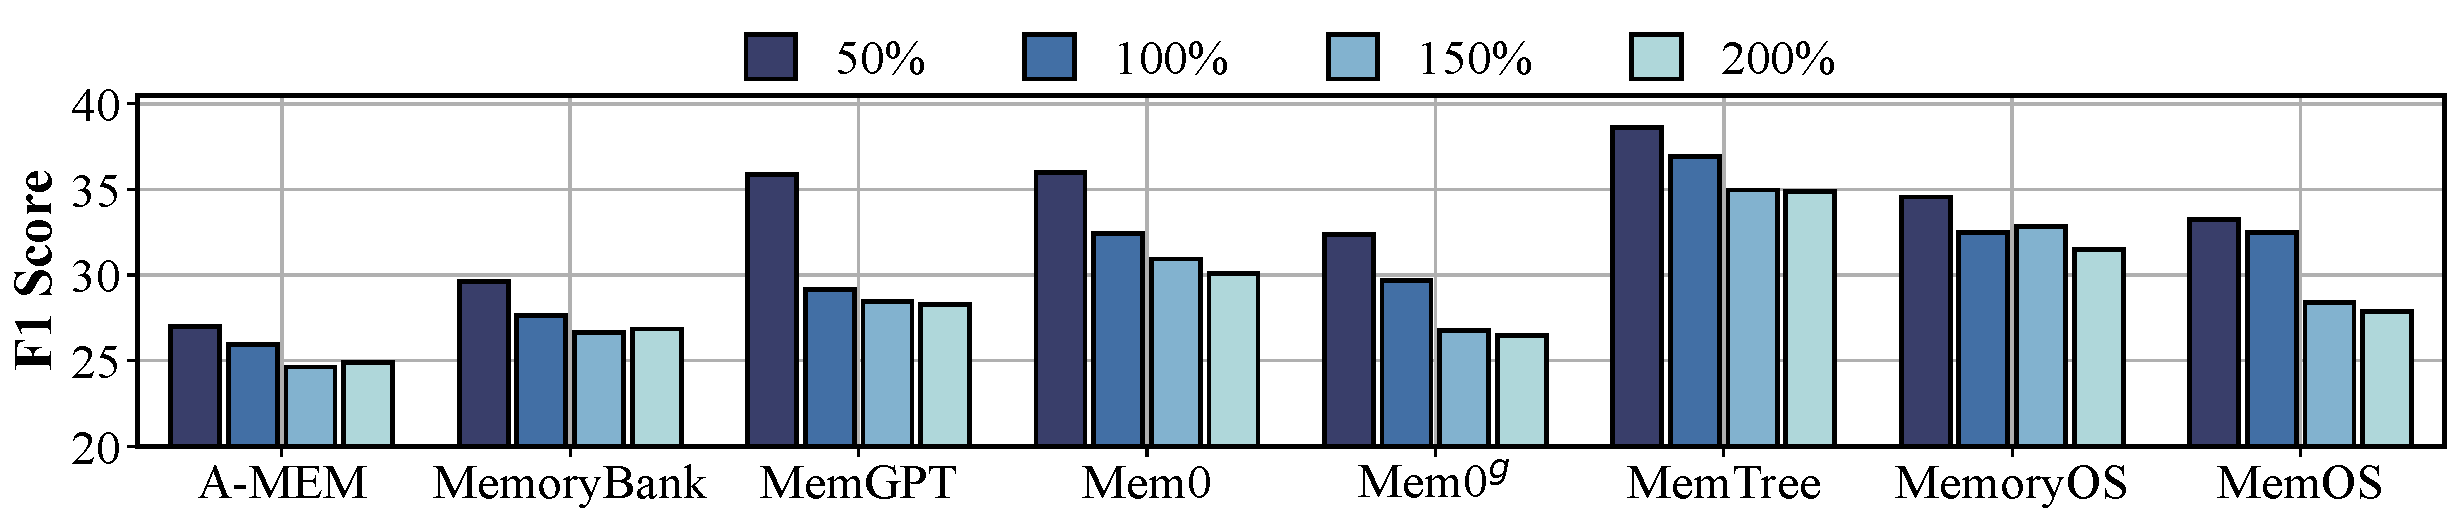
\includegraphics[width=\linewidth]{figures/scale_overall.pdf}
        \caption{Context scalability}
        \label{fig:scale_overall}
    \end{subfigure}
    
    \begin{subfigure}[]{0.85\linewidth}
        \centering
        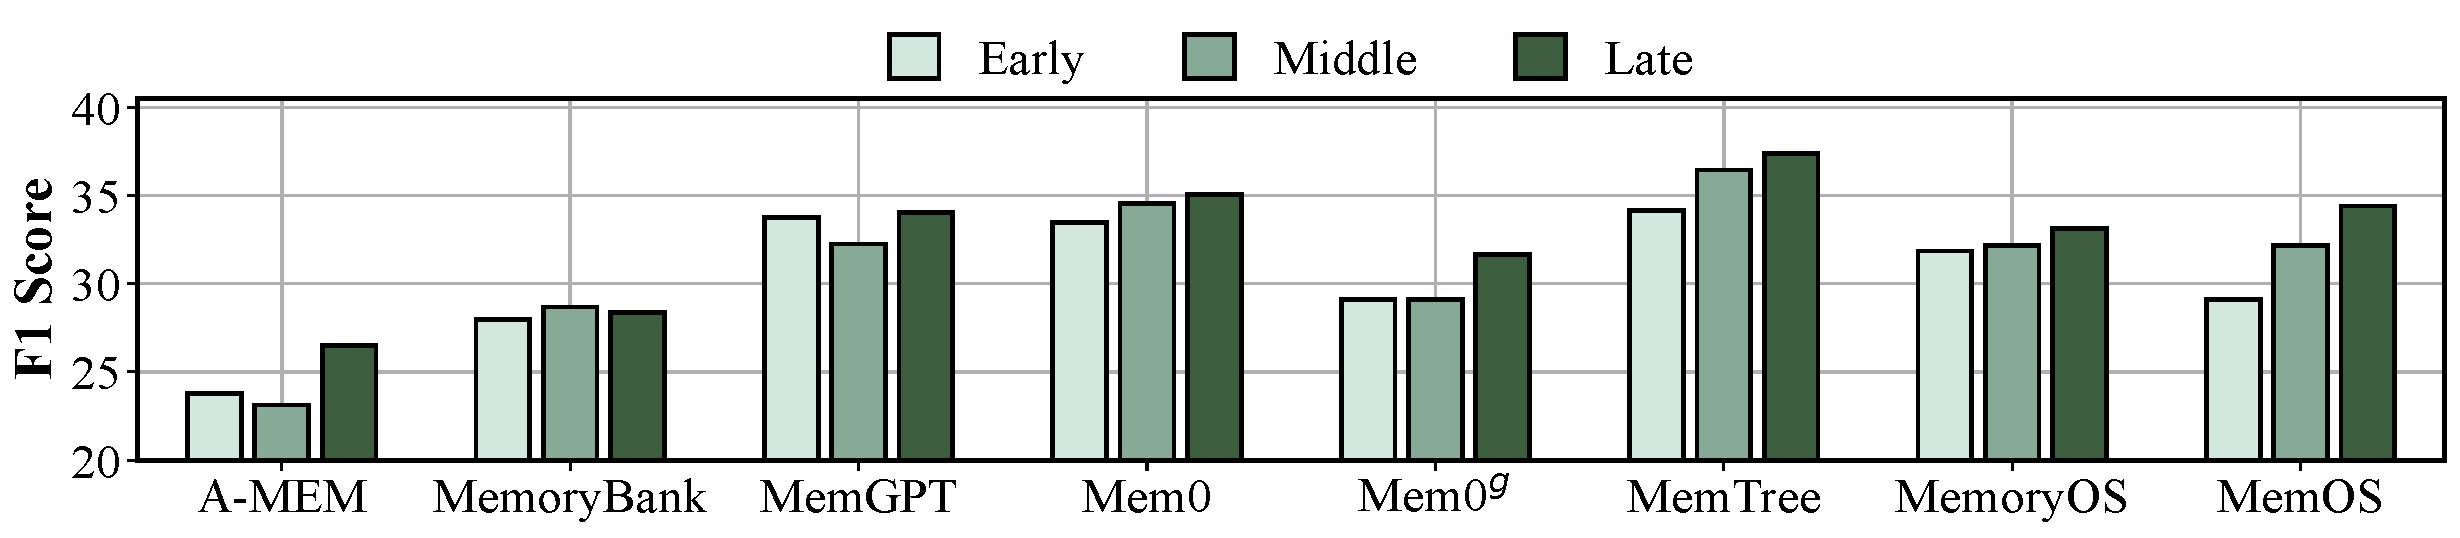
\includegraphics[width=\linewidth]{figures/position_overall.pdf}
        \caption{Position sensitivity}
        \label{fig:position_overall}
    \end{subfigure}

    \caption{Robustness analysis of memory mechanisms on LONGMEMEVAL. (a) illustrates the context scalability as the input scale varies from 50\% to 200\%, while (b) shows the position sensitivity regarding ground-truth information placed at different relative positions: Early (first 1/3), Middle (middle 1/3), and Late (last 1/3).}
    \label{fig:robustness_overall}
\end{figure*}



\begin{tikzpicture}
\filldraw (0,0) -- (-0.15,0.08) -- (-0.15,-0.08) -- cycle ; 
\end{tikzpicture} \textbf{Exp.2. Token cost analysis.}
% In this experiment, we evaluate the computational overhead for each method from two perspectives: (1) we analyze the overall trade-off between performance and cost. Figure \ref{fig:tradeoff} illustrates the relationship between the average token cost per dialogue (Y-axis) and the overall F1 Score performance (X-axis); (2) we examine the scalability of each method during the memory ingestion phase. Figure \ref{fig:token} shows how the average token consumption evolves as the volume of ingested memory increases. Based on the results, we have the following observations:
In this experiment, we evaluate the computational overhead of each method from two perspectives: (1) we analyze the overall trade-off between performance and cost. Figure~\ref{fig:tradeoff} illustrates the relationship between the average token cost per dialogue (Y-axis) and the overall F1 score (X-axis); (2) we examine the scalability of each method during the memory ingestion phase. Figure~\ref{fig:token} shows how the average token consumption evolves as the volume of ingested memory increases. Based on these results, we make the following observations:


% (1) In general, higher performance scores correlate with increased token consumption, reflecting the benefit of extensive LLM utilization. However, the design of the memory framework remains the primary determinant of cost-efficiency. Specifically, while \texttt{MemTree} and \texttt{MEMOS} achieve high accuracy, they suffer from substantial token overhead. In contrast, \texttt{MemoryOS} maintains a competitive balance, achieving high performance with significantly lower token cost. Simpler methods like \texttt{MemoChat} and \texttt{MemoryBank} minimize token usage but fail to provide adequate accuracy. Notably, while both \texttt{MemGPT} and \texttt{MemOS} are inspired by operating systems and utilize agent-based updates to autonomously decide which operations to apply, \texttt{MemOS} allocates more tokens to sophisticated decision-making, yielding better performance compared to \texttt{MemGPT}.

(1) In general, higher performance correlates with increased token consumption, reflecting the benefit of extensive LLM utilization. However, the design of the memory framework remains the primary determinant of cost efficiency. While {\tt MemTree} and {\tt MemOS} achieve high accuracy, they incur substantial token overhead. In contrast, {\tt MemoryOS} maintains a competitive balance, achieving strong performance with significantly lower token cost. Simpler methods such as {\tt MemoChat} and {\tt MemoryBank} minimize token usage but fail to deliver adequate accuracy. Notably, although both {\tt MemGPT} and {\tt MemOS} are inspired by operating systems and employ agent-based updates to autonomously decide which operations to apply, {\tt MemOS} allocates more tokens to sophisticated decision-making, yielding superior performance compared to {\tt MemGPT}.


% (2) The granularity of information processing significantly influences the token cost. Specifically, during the information extraction phase, this is defined by whether information is extracted from individual dialogue turns or collectively from multiple turns. For instance, \texttt{MemoryOS} organizes dialogues into segments for mid-term storage, while \texttt{MemoryBank} compiles historical messages into summaries at a daily granularity. Due to the strong reasoning capabilities of modern LLMs, such coarsening of granularity does not necessarily compromise performance and may even improve it, offering a viable path for enhancing memory efficiency.

(2) The granularity of information processing significantly influences token cost. During the information extraction phase, this granularity is determined by whether information is extracted from individual dialogue turns or collectively from multiple turns. For instance, {\tt MemoryOS} organizes dialogues into segments for mid-term storage, while {\tt MemoryBank} compiles historical messages into summaries at a daily granularity. Owing to the strong reasoning capabilities of modern LLMs, such coarsening of granularity does not necessarily compromise performance and may even improve it, offering a viable path toward enhancing memory efficiency.


(3) As memory volume grows, certain methods exhibit poor scalability in terms of average token cost. For {\tt MemTree}, the cost of processing each turn escalates as the tree depth increases with the accumulated dialogue history, since every top-down insertion of a new dialogue node requires updating all nodes along the path. Similarly, the graph complexity of {\tt Zep} grows with the number of dialogue turns, leading to rising costs for deduplication and consistency maintenance.




% \begin{tikzpicture}
% \filldraw (0,0) -- (-0.15,0.08) -- (-0.15,-0.08) -- cycle ; 
% \end{tikzpicture} \textbf{Exp.3. Scaling resilience analysis.}
% The scaling resilience of various memory architectures is investigated by expanding the context scale from $50\%$ to $200\%$. As shown in table/figure ?(bar plot), a consistent performance-capacity trade off exists: F1 and BLUE-1 scores decrease by $15\%$ to $30\%$ as data volume increase by $4\times$. This confirms that retrieval noise brought by larger data volume often grows faster than the model's processing capacity. The following analysis decomposes this degration across four task categories to identify the structural limits of current memory systems. 

% \textit{Information Extraction (IE):} Experimental results in this category reveal a semantic saturation effect. For flat structures like \texttt{A-MEM}, F1 and BLUE-1 decline almost linearly, indicating that increased memory density diminishes the discriminability between semantically proximal entries and leads to retrieval interference. Notably, BLEU-1 scores for \texttt{MemGPT} and \texttt{MemoryOS} decline more sharply than their F1 scores. This gap indicates that while the systems can locate the correct semantic vicinity, the increased noise at higher scales compromises exact lexical retrieval. In short, the models can identify the relevant context but struggle to extract the precise factual tokens.
% % However, structured methods like \texttt{MemTree} and \texttt{Mem0$^g$} show flatter decay curves than flat vector-based approaches

% \textit{Multi-Session Reasoning (MR):} This task identifies a complexity bottleneck in agent-managed systems. While \texttt{MemGPT} and \texttt{Mem0} perform well at $50\%$ scale, their F1 scores drop sharply beyond the $100\%$ threshold, likely due to increased retrieval interference in flat metadata. In contrast, \texttt{MemTree} exhibits superior scaling stability, with its 200\% F1 score ($27.04$) remaining competitive with its initial baseline. This resilience is attributed to its hierarchical-to-raw structure: while the bottom-level leaf nodes (raw dialogues) become dense, the higher-level summary nodes provide a condensed and stable retrieval path. This tiered architecture ensures that long-range logic remains accessible through abstract summaries even when the underlying raw sessions become cluttered at larger scales.

% \textit{Temporal Reasoning (TR):} TR is the most resilient dimension due to temporal anchoring. Unlike semantic facts that blur as the database expands, temporal data is tied to explicit sequential markers (e.g., timestamps, "before", "after") which possess high discriminability. Across all methods, F1 remains remarkably stable; \texttt{Mem0$^g$} fluctuates by less than $1\%$ between $50\%$ and $200\%$ scales. This stability proves that structural sequence provides a fixed reference, making it more resistant to scaling noise than pure semantic similarity.


% \textit{Knowledge Update (KU):} This category is the most sensitive to scaling, as increasing data volume directly elevates conflict density. For instance, \texttt{MemGPT}'s F1 score drops significantly ($40.04 \to 24.79$), suggesting that as the search space expands, the system struggles to resolve contradictions between stale and updated information. This degradation occurs because conflicting entries for the same entity occupy overlapping regions in the embedding space; at $200\%$ scale, the increased volume of historical noise frequently dilutes the relative rank of the most recent update. In contrast, \texttt{MemTree} maintains a superior F1 of $47.34$, likely because its hierarchical summarization process functions as a natural version-filtering mechanism, where higher-level nodes prioritize consolidated, up-to-date states over fragmented historical data.


% \begin{tikzpicture}
% \filldraw (0,0) -- (-0.15,0.08) -- (-0.15,-0.08) -- cycle ; 
% \end{tikzpicture} \textbf{Exp.4. Position sensitivity analysis.}
% In this experiment, we investigate how the temporal placement of key evidence affects memory retrieval and reasoning using the LONGMEMEVAL dataset. As shown in table/figure ?(bar plot), performance is not uniform across early, middle, and late evidence sessions, revealing structural biases in how different memory architectures navigate historical data. 

% \textit{Information Extraction (IE):}  While the recency bias is overall mild, its impact varies significantly across architectures. In sophisticated systems like \texttt{MemoryOS}, the assistant-side F1 only shifts from $61.32$ (early) to $63.44$ (late), indicating robust semantic stability. However, the performance gradient is far more pronounced in baseline methods such as \texttt{A-MEM}, where user-side F1 plunges from $50.84$ in late sessions to $41.62$ in early sessions. This drastic decay suggests that in systems with continuous update or evolving memory buffers, older evidence is susceptible to semantic erosion: as new sessions are indexed, the feature representations of distant memories are increasingly diluted by accumulated noise or partially overwritten, leading to a failure in precise token extraction for early-session facts.

% \textit{Multi-Session Reasoning (MR):} This dimension demonstrates the most consistent sensitivity to evidence placement. Across most architectures, there is a clear performance gradient: \texttt{MemTree} improves from an F1 of $26.18$ (early) to $27.45$ (late), and \texttt{MemoryOS} climbs from $19.35$ to $22.18$. This confirms that maintaining reasoning chains is structurally easier when the logical "hops" between the evidence and the query are minimized. As the temporal distance increases, the risk of the reasoning chain fracturing due to accumulated metadata noise in earlier sessions becomes more pronounced.

% \textit{Temporal Reasoning (TR):} As in the last experiment, This capability demonstrates the strongest positional resilience. Most methods maintain stable performance with fluctuations typically within 
% 3 F1 points.  Notably, Mem0$_g$ shows exceptional stability (27.88$\rightarrow$27.70
% $\rightarrow$28.61, variance $<$ 1 F1 point), and MemOS also exhibits strong consistency 
% (22.12$\rightarrow$23.58$\rightarrow$23.33). This robustness can be attributed to their 
% structural advantages:  Mem0$_g$'s graph-based storage explicitly preserves temporal 
% attributes as node properties, enabling structure-based retrieval that bypasses 
% position-dependent semantic drift; MemOS's hierarchical summarization retains temporal 
% markers across abstraction levels, ensuring temporal anchors remain accessible regardless 
% of evidence depth.  These results confirm that temporal queries benefit from explicit 
% structural encoding rather than relying solely on semantic similarity.



% \textit{Knowledge Update (KU):} The recency bias is highly evident in KU, but the degree of sensitivity depends on the conflict-resolution mechanism. Systems like \texttt{Mem0} and \texttt{MemoryOS} show a clear performance gain in late sessions (34.98→42.04 and 30.62→38.39, respectively), as recent updates are less likely to be overshadowed by subsequent historical noise. In contrast, \texttt{MemTree} maintains a high and stable F1 score (around 40 percent) across all positions, demonstrating that its hierarchical summarization effectively "locks" updated states regardless of their depth. The performance of \texttt{A-MEM} also remained strong from early to late sessions. 




% \begin{tikzpicture}
% \filldraw (0,0) -- (-0.15,0.08) -- (-0.15,-0.08) -- cycle ; 
% \end{tikzpicture} \textbf{Exp.3. Scaling resilience analysis.}
% The scaling resilience of various memory architectures is investigated by expanding the context scale from $50\%$ to $200\%$. As shown in table/figure ?(bar plot), a consistent performance-capacity trade off exists: F1 and BLUE-1 scores decrease by $15\%$ to $30\%$ as data volume increase by $4\times$. This confirms that retrieval noise brought by larger data volume often grows faster than the model's processing capacity. The following analysis decomposes this degration across four task categories to identify the structural limits of current memory systems. 

% \textit{Information Extraction (IE):} Experimental results in this category reveal a semantic saturation effect. For flat structures like \texttt{A-MEM}, F1 and BLUE-1 decline almost linearly, indicating that increased memory density diminishes the discriminability between semantically proximal entries and leads to retrieval interference. Notably, BLEU-1 scores for \texttt{MemGPT} and \texttt{MemoryOS} decline more sharply than their F1 scores. This gap indicates that while the systems can locate the correct semantic vicinity, the increased noise at higher scales compromises exact lexical retrieval. In short, the models can identify the relevant context but struggle to extract the precise factual tokens.
% % However, structured methods like \texttt{MemTree} and \texttt{Mem0$^g$} show flatter decay curves than flat vector-based approaches

% \textit{Multi-Session Reasoning (MR):} This task identifies a complexity bottleneck in agent-managed systems. While \texttt{MemGPT} and \texttt{Mem0} perform well at $50\%$ scale, their F1 scores drop sharply beyond the $100\%$ threshold, likely due to increased retrieval interference in flat metadata. In contrast, \texttt{MemTree} exhibits superior scaling stability, with its 200\% F1 score ($27.04$) remaining competitive with its initial baseline. This resilience is attributed to its hierarchical-to-raw structure: while the bottom-level leaf nodes (raw dialogues) become dense, the higher-level summary nodes provide a condensed and stable retrieval path. This tiered architecture ensures that long-range logic remains accessible through abstract summaries even when the underlying raw sessions become cluttered at larger scales.

% \textit{Temporal Reasoning (TR):} TR is the most resilient dimension due to temporal anchoring. Unlike semantic facts that blur as the database expands, temporal data is tied to explicit sequential markers (e.g., timestamps, "before", "after") which possess high discriminability. Across all methods, F1 remains remarkably stable; \texttt{Mem0$^g$} fluctuates by less than $1\%$ between $50\%$ and $200\%$ scales. This stability proves that structural sequence provides a fixed reference, making it more resistant to scaling noise than pure semantic similarity.


% \textit{Knowledge Update (KU):} This category is the most sensitive to scaling, as increasing data volume directly elevates conflict density. For instance, \texttt{MemGPT}'s F1 score drops significantly ($40.04 \to 24.79$), suggesting that as the search space expands, the system struggles to resolve contradictions between stale and updated information. This degradation occurs because conflicting entries for the same entity occupy overlapping regions in the embedding space; at $200\%$ scale, the increased volume of historical noise frequently dilutes the relative rank of the most recent update. In contrast, \texttt{MemTree} maintains a superior F1 of $47.34$, likely because its hierarchical summarization process functions as a natural version-filtering mechanism, where higher-level nodes prioritize consolidated, up-to-date states over fragmented historical data.

% \begin{figure*}[]
%     \centering
%     \setlength{\abovecaptionskip}{0.1cm}
%     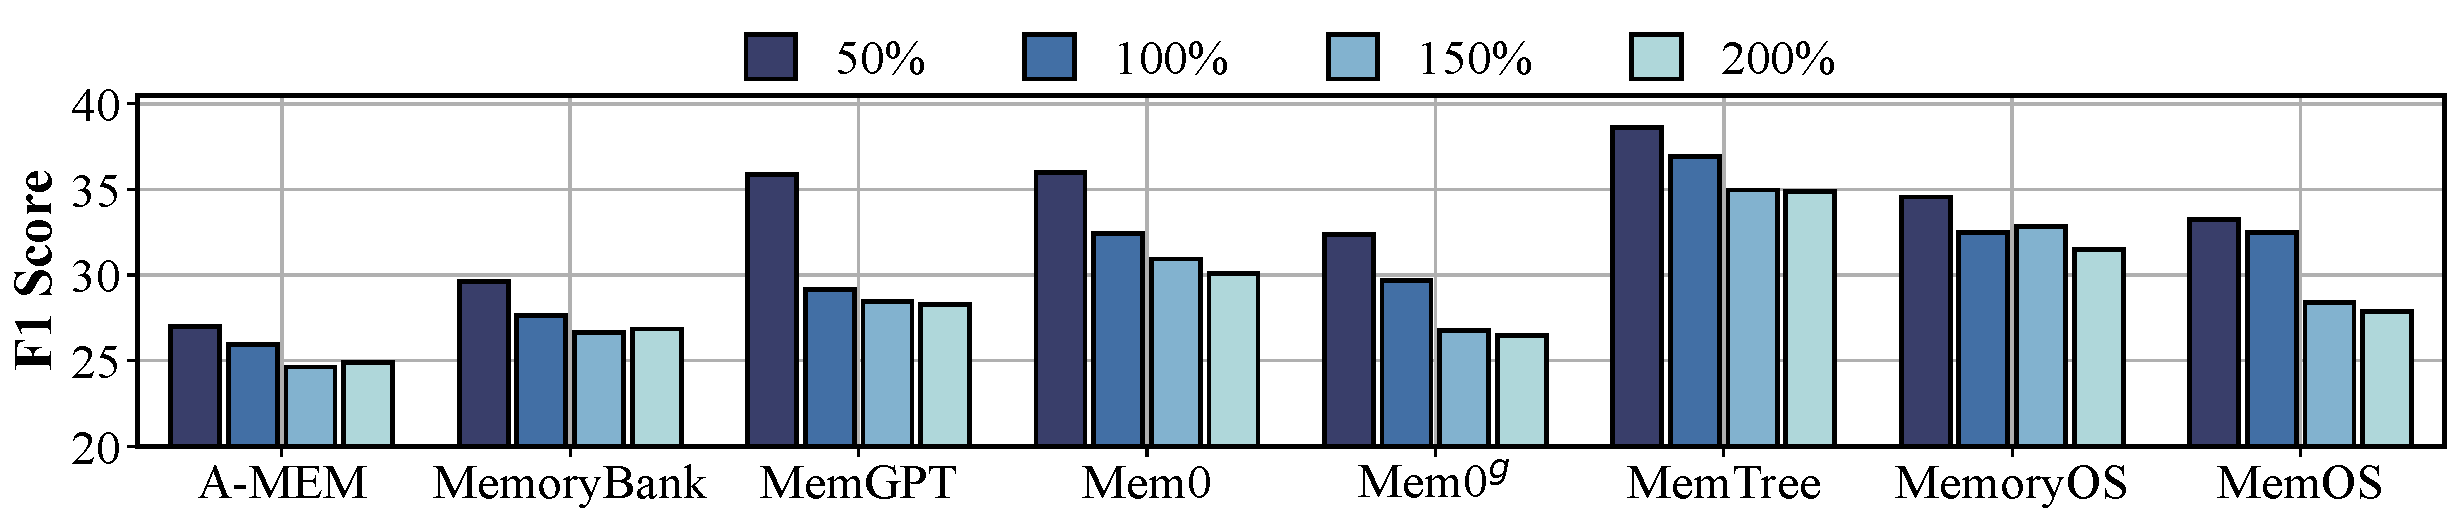
\includegraphics[width=0.85\linewidth]{figures/scale_overall.pdf}
%     \caption{Performance comparison of methods across varying context lengths on LONGMEMEVAL.}
%     \label{fig:scale_overall}
% \end{figure*}

% \begin{figure*}[]
%     \centering
%     \setlength{\abovecaptionskip}{0.1cm}
%     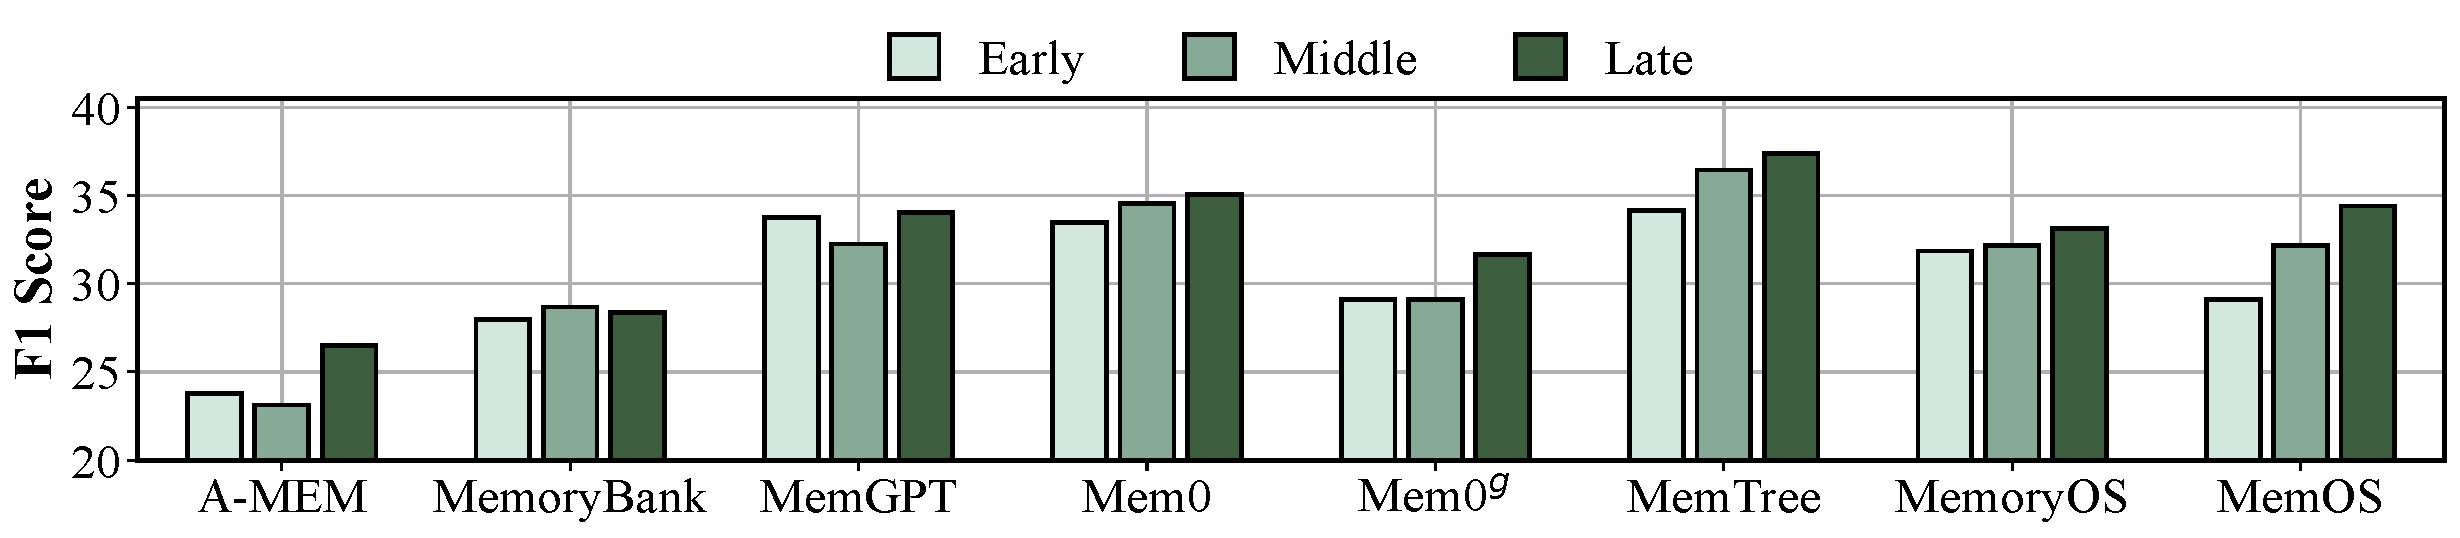
\includegraphics[width=0.85\linewidth]{figures/position_overall.pdf}
%     \caption{Performance comparison of methods across varying context lengths on LONGMEMEVAL.}
%     \label{fig:position_overall}
% \end{figure*}





\begin{tikzpicture}
\filldraw (0,0) -- (-0.15,0.08) -- (-0.15,-0.08) -- cycle ; 
\end{tikzpicture} \textbf{Exp.3. Context scalability analysis.}\label{exp3}
% The scaling resilience of various memory architectures is investigated by expanding the context scale from $50\%$ to $200\%$. As shown in table/figure ?(bar plot), a consistent performance-capacity trade off exists: F1 and BLUE-1 scores decrease by $15\%$ to $30\%$ as data volume increase by $4\times$. This confirms that retrieval noise brought by larger data volume often grows faster than the model's processing capacity. The following analysis decomposes this degration across four task categories to identify the structural limits of current memory systems. 
% The context scalability of various memory architectures is investigated by expanding the context scale from $50\%$ to $200\%$. In long-horizon interactions, the primary challenge for memory systems shifts from simple retrieval to robust suppression of noise as the information density grows. By subjecting diverse architectures to this scaling pressure, we identify their operational ceilings—specifically how different structural designs maintain retrieval precision despite the performance-degrading effects of increased context scale. The following analysis highlights the structural limits and strengths of current memory systems in achieving context scalability:
In this experiment, we investigate the context scalability of various memory architectures by expanding the context length of LONGMEMEVAL from $50\%$ to $200\%$. In long-horizon interactions, the primary challenge for memory systems shifts from simple retrieval to robust noise suppression as information density grows. 
We evaluate various architectures across different context sizes to see how well they maintain retrieval precision as context grows.
Figure~\ref{fig:scale_overall} illustrates the overall trends in context scalability, while comprehensive experimental results are detailed in Appendix ~\ref{sec:app:exp:result}.
% By subjecting diverse architectures to this scaling pressure, we identify their operational ceilings---specifically, how different structural designs maintain retrieval precision despite the performance degradation induced by increased context scale. Detailed experimental results are provided in Appendix~\ref{sec:app:exp:result}. And the key findings are summarized below:


% The following analysis identifies the structural limits and strength of current memory systems in context scalability.  

\begin{figure}[h]
    \centering
    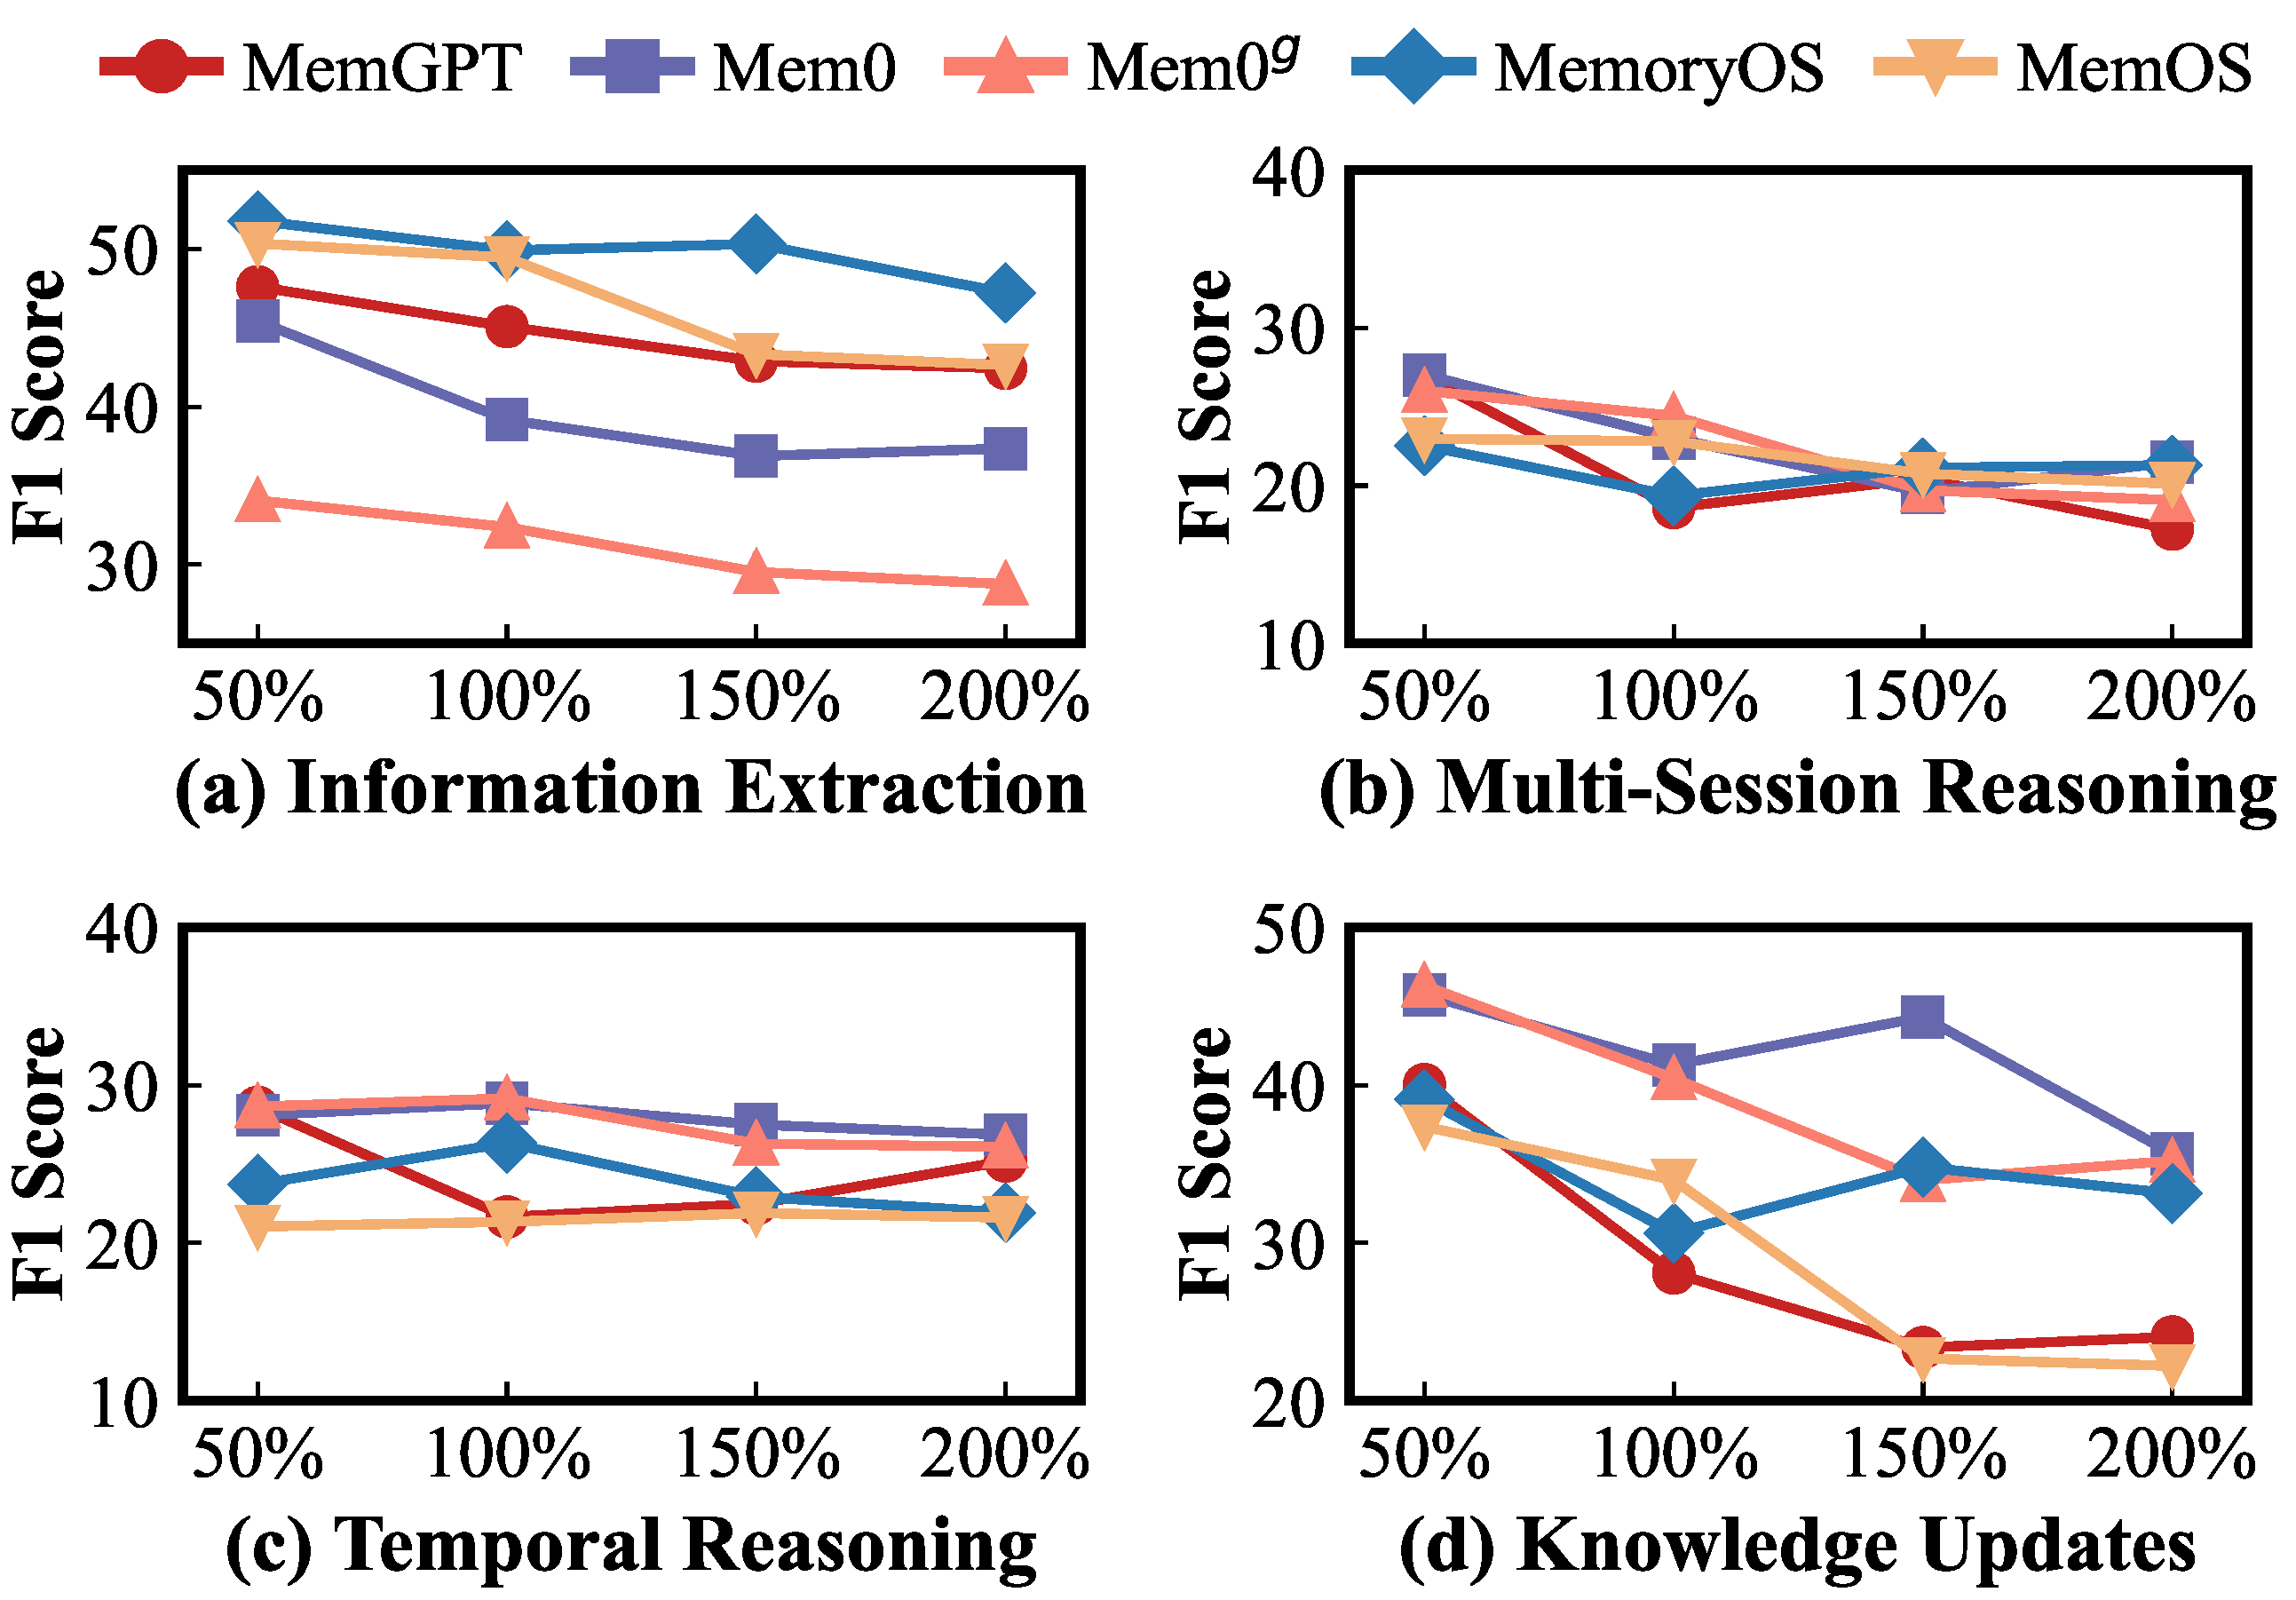
\includegraphics[width=1.0\linewidth]{figures/scale_tasks.pdf}
    \caption{Context scalability of various memory methods across different task categories on LONGMEMEVAL.}
    \label{fig:scale_tasks}
\end{figure}


%TODO: 

% (1) As shown in table/figure ?(bar plot), a consistent performance-capacity trade off exists: F1 and BLUE-1 scores decrease by $15\%$ to $30\%$ as data volume increase by $4\times$. This confirms that retrieval noise brought by larger data volume often grows faster than the model's processing capacity. 

(1) As the context scale expands from $50\%$ to $200\%$, nearly all memory architectures exhibit a steady decline in F1 scores. This performance attrition is primarily driven by the increased density of irrelevant information, which lowers the signal-to-noise ratio during retrieval. 

% However, the performance curves for {\tt Memtree} and {\tt MemoryOS} remain notably flatter than their counterparts, demonstrating superior scaling resilience. This indicates that structured indexing can effectively mitigate the interference caused by a larger search space.

(2) The scaling results reveal a performance divide rooted in operational complexity. Methods such as {\tt MemOS} and {\tt MemGPT} implement an ``LLM-as-OS'' paradigm, requiring the LLM to autonomously manage memory via complex tool calls. As the scale increases to $200\%$, the expanded candidate space significantly raises the difficulty for the LLM to accurately reason over and execute these management instructions, leading to higher rates of tool-call failures and indexing conflicts. In contrast, {\tt MemoryOS} reduces the agent's cognitive load by employing explicit rule-based hierarchical management. By offloading organizational logic from the LLM to a deterministic framework, {\tt MemoryOS} maintains high stability, demonstrating that simplifying the agent's internal management overhead through deliberate design is critical for robust scaling.


(3) Different task categories exhibit varying sensitivity to scaling pressure. As illustrated in Figure~\ref{fig:scale_tasks}, Knowledge Update (KU) is particularly sensitive, showing sharp performance attrition because an increased memory volume raises the density of conflicting records. Since KU requires the model to identify the latest fact among mutually exclusive versions, the presence of more obsolete candidates directly increases retrieval interference. Conversely, temporal tasks remain relatively stable, as they rely on the relative ordering of events, which remains structurally distinct even as the background volume grows. Unlike the versioning conflicts in KU, the chronological precedence of events is not easily compromised by the addition of context.


% (2) The scaling results highlight a sharp divide between architectural designs. Systems such as {\tt MemOS} and {\tt MemGPT} are more susceptible to performance collapse at larger scale, as their reliance on monolithic buffers or flatter structures leads to severe indexing conflicts and retrieval noise. In contrast, {\tt MemoryOS} maintains significantly higher stability. By decoupling information into hierarchical layers, it successfully bypasses the structural limits that plague single-dimensional storage, proving that hierarchical management is essential for resilient scaling.

% The following analysis decomposes this degration across four task categories to identify the structural limits of current memory systems. 

% \textit{Information Extraction (IE):} Experimental results in this category reveal a semantic saturation effect. For flat structures like \texttt{A-MEM}, F1 and BLUE-1 decline almost linearly, indicating that increased memory density diminishes the discriminability between semantically proximal entries and leads to retrieval interference. Notably, BLEU-1 scores for \texttt{MemGPT} and \texttt{MemoryOS} decline more sharply than their F1 scores. This gap indicates that while the systems can locate the correct semantic vicinity, the increased noise at higher scales compromises exact lexical retrieval. In short, the models can identify the relevant context but struggle to extract the precise factual tokens.
% % However, structured methods like \texttt{MemTree} and \texttt{Mem0$^g$} show flatter decay curves than flat vector-based approaches

% \textit{Multi-Session Reasoning (MR):} This task identifies a complexity bottleneck in agent-managed systems. While \texttt{MemGPT} and \texttt{Mem0} perform well at $50\%$ scale, their F1 scores drop sharply beyond the $100\%$ threshold, likely due to increased retrieval interference in flat metadata. In contrast, \texttt{MemTree} exhibits superior scaling stability, with its 200\% F1 score ($27.04$) remaining competitive with its initial baseline. This resilience is attributed to its hierarchical-to-raw structure: while the bottom-level leaf nodes (raw dialogues) become dense, the higher-level summary nodes provide a condensed and stable retrieval path. This tiered architecture ensures that long-range logic remains accessible through abstract summaries even when the underlying raw sessions become cluttered at larger scales.

% \textit{Temporal Reasoning (TR):} TR is the most resilient dimension due to temporal anchoring. Unlike semantic facts that blur as the database expands, temporal data is tied to explicit sequential markers (e.g., timestamps, "before", "after") which possess high discriminability. Across all methods, F1 remains remarkably stable; \texttt{Mem0$^g$} fluctuates by less than $1\%$ between $50\%$ and $200\%$ scales. This stability proves that structural sequence provides a fixed reference, making it more resistant to scaling noise than pure semantic similarity.


% \textit{Knowledge Update (KU):} This category is the most sensitive to scaling, as increasing data volume directly elevates conflict density. For instance, \texttt{MemGPT}'s F1 score drops significantly ($40.04 \to 24.79$), suggesting that as the search space expands, the system struggles to resolve contradictions between stale and updated information. This degradation occurs because conflicting entries for the same entity occupy overlapping regions in the embedding space; at $200\%$ scale, the increased volume of historical noise frequently dilutes the relative rank of the most recent update. In contrast, \texttt{MemTree} maintains a superior F1 of $47.34$, likely because its hierarchical summarization process functions as a natural version-filtering mechanism, where higher-level nodes prioritize consolidated, up-to-date states over fragmented historical data.



\begin{table}[t]
\centering
\caption{Position sensitivity analysis of representative memory mechanisms across Information Extraction sub-tasks on LONGMEMEVAL (F1 Score).}
\small
\begin{tabular}{llrrr}
\toprule

{\textbf{Method}} & {\textbf{Position}} & \textbf{user} & \textbf{assistant} & \textbf{preference} \\
\midrule

\multicolumn{1}{l}{\multirow{4}{*}{\tt Mem0$^g$}} & Early & 53.95 & 19.62 & 9.93\\
& Middle &48.88 & 17.02 & 10.52\\
& Late & 63.48 & 17.91 & 11.01 \\
\cline{2-5}
& Improvement & \textbf{\textcolor{green!60!black}{+9.53}} & \textbf{\textcolor{red}{-1.71}} & \textbf{\textcolor{green!60!black}{+1.08}} \\
\midrule

\multicolumn{1}{l}{\multirow{4}{*}{\tt MemTree}} & Early & 52.85 & 49.26 & 9.31 \\
& Middle & 60.03 & 60.82 & 10.58 \\
& Late & 63.59 & 58.18 & 9.72 \\
\cline{2-5}
& Improvement & \textbf{\textcolor{green!60!black}{+10.74}} & \textbf{\textcolor{green!60!black}{+8.92}} & \textbf{\textcolor{green!60!black}{+0.41}} \\
\midrule

\multicolumn{1}{l}{\multirow{4}{*}{\tt MemOS}} & Early & 60.65 & 43.00 & 11.20 \\
& Middle & 64.24 & 49.26 & 11.97 \\
& Late & 69.88 & 51.30 & 11.86 \\
\cline{2-5}
& Improvement & \textbf{\textcolor{green!60!black}{+9.23}} & \textbf{\textcolor{green!60!black}{+8.30}} & \textbf{\textcolor{green!60!black}{+0.66}} \\
\bottomrule

\label{tab:pos_IE}
\end{tabular}
\end{table}


\begin{tikzpicture}
\filldraw (0,0) -- (-0.15,0.08) -- (-0.15,-0.08) -- cycle ; 
\end{tikzpicture} 
\textbf{Exp.4. Position sensitivity analysis.}
% In this experiment, we investigate how the temporal placement of key evidence affects memory retrieval and reasoning using the LONGMEMEVAL dataset. Distinct from the scaling analysis that focuses on information density, this experiment evaluates positional sensitivity by manipulating the temporal placement of key evidence relative to the query. The fundamental challenge here is the interference of intervening context: as the evidence is placed earlier in the timeline, the system must bridge a wider "temporal gap" and resist the distraction of subsequent dialogue turns. This analysis identifies whether architectural designs exhibit temporal invariance—maintaining equal accessibility to historical records—or if they suffer from structural biases that favor recent inputs over distant evidence. As shown in table/figure ?(bar plot), performance is not uniform across early, middle, and late evidence sessions, revealing structural biases in how different memory architectures navigate historical data. 
% In this experiment, we investigate how the temporal placement of key evidence affects memory retrieval and reasoning on the variant dataset of LONGMEMEVAL. Unlike the scaling analysis in Exp3, which focuses on information density, this experiment evaluates positional sensitivity by manipulating the location of key evidence relative to the query. The fundamental challenge lies in the interference of intervening context: as evidence is placed earlier in the timeline, the system must bridge a wider temporal gap and resist distraction from subsequent dialogue turns. This analysis aims to determine whether architectural designs exhibit temporal invariance---maintaining equal accessibility to historical records---or suffer from structural biases that favor recent inputs over distant evidence. As shown in Figure~\ref{fig:position_overall}, performance is not uniform across early, middle, and late evidence placements, revealing structural biases in how different memory architectures navigate historical data. Complete experimental outcomes can be found in  Appendix~\ref{sec:app:exp:result} Table~\ref{tab:lmepos} and the key findings are as follows:
In this experiment, we evaluate how the placement of key evidence affects retrieval and reasoning on variants of LONGMEMEVAL by positioning the evidence in the early (first 1/3), middle (middle 1/3), or late (last 1/3) sections of the context. As evidence appears earlier in the context, memory systems must bridge larger temporal gaps and handle increased interference from subsequent dialogue. This experiment tests whether architectures maintain uniform access to historical records or exhibit a bias toward recent inputs. As illustrated in Figure~\ref{fig:position_overall}, performance varies significantly across early, middle, and late placements. 
Detailed results are provided in Appendix~\ref{sec:app:exp:result}, and the key findings are summarized as follows:



% (1) A universal performance degradation is observed as the temporal distance between the evidence and the query increases. Most methods exhibit a pronounced ``recency bias,'' with performance in Late sessions significantly exceeding that in Early sessions. This trend is most evident in complex reasoning tasks. For instance, A-mem improves from F1 scores in early sessions to F1 scores in late sessions, while MemOS improves from \revise{[TODO: add specific examples]} This finding suggests that as the dialogue history grows, maintaining long-range information consistency and retrieval accuracy becomes increasingly challenging.

% (1) A universal performance degradation is observed as the temporal distance between the evidence and the query increases. To be more specific, most methods exhibit a pronounced "recency bias", with performance in Late sessions exceeding that in Early sessions. This trend is most evident in complex reasoning tasks. For instance, in the multi-session reasoning category in Table \ref{tab:lmepos}, A-mem improves from 20.31 F1 scores in early sessions to 24.63 F1 scores in late sessions, while MemOS improves from 22.12 to 26.25. \revise{[Added: add specific examples]} This finding suggests that as the dialogue history grows, maintaining long-range information consistency and retrieval accuracy becomes increasingly challenging.

(1) A clear recency bias is observed at the overall level as the temporal distance between supporting evidence and the query increases. As shown in Figure~\ref{fig:position_overall}, most methods achieve higher overall F1 scores when the evidence is placed in late sessions rather than early sessions. That is, the overall F1 score improves from 34.13 to 37.37 for \texttt{MemTree}, from 29.10 to 34.40 for \texttt{MemOS}, etc.
As more intervening dialogue accumulates after the relevant evidence appears, maintaining long-range information consistency and retrieval becomes increasingly challenging. 

%TODO: Check table 10 for numbers
% may focus on the overall perfrmance without focusing on specific categories

% (2) The mechanism of memory updating is crucial to preserving historical information and avoiding "memory overwriting." We observe that models like {\tt A-MEM}, which rely on dynamic updates that may partially overwrite older states to stay current, show a disproportionate performance gap between Late and Early sessions (e.g.). In contrast, tree-based or hierarchical structures such as {\tt Memtree} and {\tt MemoryOS} implement updates that assign higher priority to new information without discarding the old. This structured approach allows them to maintain relatively stable performance across all positions, effectively "locking" historical evidence against the interference of subsequent sessions.

% (2) The mechanism of memory updating is crucial to preserving historical information and preventing memory overwriting. Models such as {\tt A-MEM}, which rely on dynamic updates that may partially overwrite older states to stay current, exhibit a disproportionate performance gap between Late and Early sessions. \revise{[TODO: add specific numbers]}
% In contrast, tree-based or hierarchical structures such as {\tt MemTree} and {\tt MemoryOS} implement updates that assign higher priority to new information without discarding the old. This structured approach enables them to maintain relatively stable performance across all positions, effectively preserving historical evidence against the interference of subsequent sessions.
% (2) The mechanism of memory updating is crucial to preserving historical information and preventing memory overwriting. Models such as {\tt A-MEM}, which rely on dynamic updates that may partially overwrite older states to stay current, exhibit a disproportionate performance gap between Late and Early sessions. \revise{[TODO: add specific numbers]}
% Meanwhile, tree-based or hierarchical structures such as {\tt MemTree} and {\tt MemoryOS} implement updates that assign higher priority to new information. This property also leads to performance gap between late and early sessions. 

% (2) Memory update policy is an important factor affecting position sensitivity. In \texttt{A-MEM}, memory is dynamically revised over time, and later updates may partially overwrite or obscure earlier evidence, making early-session information more vulnerable to subsequent interactions. For hierachical or tree-based methods such as {\tt MemTree} and {\tt MemOS}, the effect arises differently: although the raw dialogue may still be retained at the leaf level, newly arriving information can have stronger influence on higher-level summaries as the high-level nodes are updated, thereby making recent evidence/memories more prominent in the maintained representation. By contrast, update strategies that preserve historical information in a more balanced manner appear less prone to introducing large positional positional differences. {\tt MemoryOS}, for instance, organizes updates through stage-wise transfer acorss separate memory levels. Under this design, earlier evidence can remain preserved as relatively independent content within a specific level, rather than being repeatedly merged with later information. As a result, later interactions do not always directly reshape the representation carrying earlier evidence, which helps explain why {\tt MemoryOS} exhibits a relatively smaller overall Late--Early gap (+1.29 F1). 

(2) Memory update policy significantly affects position sensitivity. For methods like \texttt{A-MEM}, dynamic memory revisions can overwrite earlier evidence, making early-session information vulnerable to later interactions. Hierarchical methods like {\tt MemTree} and {\tt MemOS} exhibit different mechanisms: although raw dialogue is retained at leaf nodes, updates to higher-level summaries amplify recent information's influence, increasing the Late–Early gap. In contrast, {\tt MemoryOS} preserves historical information more evenly through stage-wise transfers across memory levels. Earlier evidence remains relatively independent within each level rather than being repeatedly merged with later information. Consequently, later interactions do not directly reshape earlier evidence representations, explaining {\tt MemoryOS}'s smaller Late–Early gap (+1.29 F1).


% These results indicate that position sensitivity depends on  



% Models such as {\tt A-MEM}, which rely on dynamic updates that may partially overwrite older states to stay current, exhibit a disproportionate performance gap between Late and Early sessions. \revise{[TODO: add specific numbers]}
% Meanwhile, tree-based or hierarchical structures such as {\tt MemTree} and {\tt MemoryOS} implement updates that assign higher priority to new information. This property also leads to performance gap between late and early sessions. 

% a-mem: overwrite;memos/memtree:new information has more weights; *analyze update policies that may bridge the gap


% (3) The position sensitivity to evidence placement is highly category-dependent. To characterize this effect, we report three representative methods in Table~\ref{tab:pos_IE} and examine their positional variations across the information extraction sub-tasks. In general, transient, session-localized information exhibits much stronger position sensitivity than persistent traits. Particularly, the {\it user} and {\it assistant} extraction tasks show substantial Early-to-Late changes across methods (e.g., +9.53/+10.74/+9.23 for {\tt Mem0$_g$}/{\tt MemTree}/{\tt MemOS} on the user subtask, and +8.92/+8.30 for {\tt MemTree}/{\tt MemOS} on the assistant subtask). In contrast, the {\it preference} extraction task remains comparatively stable under evidence relocation: the improvements are consistently small(+1.08, +0.41, and +0.66 for {\tt Mem0$_g$}, {\tt MemTree}, and {\tt MemOS}, respectively). This indicates that position sensitivity is largely driven by the inherent persistence of information: transient session-local details suffer more from later interference, whereas distilled preference traits are less affected by evidence relocation.

(3) Position sensitivity is highly category-dependent. We examine three representative methods in Table~\ref{tab:pos_IE} across information extraction sub-tasks. Transient, session-localized information exhibits stronger position sensitivity than persistent traits. The user and assistant extraction tasks show substantial Early-to-Late changes: +9.53/+10.74/+9.23 F1 for {\tt Mem0$_g$}/{\tt MemTree}/{\tt MemOS} on user extraction, and +8.92/+8.30 F1 for {\tt MemTree}/{\tt MemOS} on assistant extraction. In contrast, preference extraction remains stable: improvements are only +1.08, +0.41, and +0.66 F1 respectively. This indicates that position sensitivity correlates with information persistence: transient session-local details suffer more from later interference, while persistent preference traits are less affected by evidence relocation.





\begin{tikzpicture}
\filldraw (0,0) -- (-0.15,0.08) -- (-0.15,-0.08) -- cycle ; 
\end{tikzpicture} 
\textbf{Exp.5. LLM backbone comparison.}
In this experiment, we evaluate several memory methods across different LLM backbones. Specifically, we select representative and high-performing methods from each design paradigm for this cross-backbone evaluation. We therefore exclude simpler baselines to focus on methods with non-trivial memory architectures. The results are presented in Table~\ref{tab:model}. 
Overall, most methods achieve their best performance with the closed-source GPT-4o-mini backbone. Among open-source models, Qwen2.5-7B generally outperforms LLaMA3.1-8B across methods, with the exception of {\tt MemoryOS}, where LLaMA3.1-8B yields better results. Scaling Qwen2.5 from 7B to 72B produces substantial gains for all memory methods, as discussed in Exp.1, indicating that existing memory architectures remain heavily dependent on the backbone's reasoning capability.



\begin{table}[]
    \centering
    \caption{Comparison across LLM backbones on LOCOMO.}
    \label{tab:model}
    \small
    \setlength{\tabcolsep}{4pt}
    \begin{threeparttable}
        \begin{tabular}{l|l|r|r|r|r|r}
        \toprule
        \textbf{Model} & Metric & \multicolumn{1}{c|}{\texttt{Zep}} & \multicolumn{1}{c|}{\texttt{MemTree}} & \multicolumn{1}{c|}{\texttt{MemoryOS}} & \multicolumn{1}{c|}{\texttt{MemOS}} & \multicolumn{1}{c}{\texttt{Ours}} \\
        \midrule
        \multirow{2}{*}{Qwen2.5-7B}
          & F1    & 33.82 & 29.68 & 28.34 & 37.05 & \textbf{38.03} \\
          & BLEU-1 & 27.42 & 23.95 & 23.11 & 30.30 & \textbf{31.73} \\
        \midrule
        \multirow{2}{*}{Qwen2.5-72B}
          & F1    & 37.45 & 34.85 & 39.63 & 42.79 & \textbf{43.87} \\
          & BLEU-1 & 30.46 & 28.49 & 32.62 & 35.16 & \textbf{37.30} \\
        \midrule
        \multirow{2}{*}{LLaMA3.1-8B}
          & F1    & ---     & 23.49 & 32.21 & 33.39 & \textbf{35.21} \\
          & BLEU-1 & ---     & 18.19 & 25.56 & 26.24 & \textbf{28.40} \\
        \midrule
        \multirow{2}{*}{GPT-4o-mini}
          & F1    & 42.88 & 32.32 & 42.57 & \textbf{45.56} & 45.20 \\
          & BLEU-1 & 36.09 & 25.89 & 34.75 & 38.06 & \textbf{38.52} \\
        \bottomrule
        \end{tabular}

        \begin{tablenotes}[flushleft]
            \small
            \item[$\dagger$]Results for \texttt{Zep} on LLaMA3.1-8B are marked as ``---'' due to strict JSON formatting failures, as noted in its official documentation\footnotemark.
        \end{tablenotes}
    \end{threeparttable}
\end{table}
\footnotetext{\url{https://help.getzep.com/graphiti/configuration/llm-configuration\#ollama-local-llms}}
% \footnotetext{\url{https://help.getzep.com/graphiti/configuration/llm-configuration}}



%%%%%% sota result

\begin{table*}[]
\centering
\caption{Comparison of our newly designed method on LONGMEMEVAL using Qwen2.5-7B-Instruct (F1 Score).}
\label{tab:sota_lme}
\small
\begin{tabular}{l|r|r|r|r|r|r|r|r|r}
\toprule
\textbf{Category} & \multicolumn{1}{c|}{\tt A-MEM} & \multicolumn{1}{c|}{\tt MemoryBank} & \multicolumn{1}{c|}{\tt MemGPT} & \multicolumn{1}{c|}{\tt Mem0} & \multicolumn{1}{c|}{\tt Mem0$^g$} & \multicolumn{1}{c|}{\tt MemTree} & \multicolumn{1}{c|}{\tt MemoryOS} & \multicolumn{1}{c|}{\tt MemOS} & \multicolumn{1}{c}{\tt Ours} \\
\midrule
Information Extraction-user & 46.75 & 46.28 & 52.82 & 56.51 & 53.21 & \fst{68.48} & 56.85 & 65.48 & \snd{67.38} \\
Information Extraction-assistant & 43.21 & 49.31 & 52.26 & 32.35 & 18.18 & 57.79 & \snd{61.32} & 49.40 & \fst{69.34} \\
Information Extraction-preference & 9.76 & \snd{13.96} & 13.61 & 11.44 & 10.23 & 9.50 & 12.40 & 12.17 & \fst{14.58} \\
Multi-Session Reasoning & 16.61 & 19.41 & 18.61 & 23.02 & \fst{24.42} & 21.96 & 19.35 & 22.81 & \snd{23.14} \\
Knowledge Update & 19.37 & 17.80 & 21.65 & 28.86 & 29.16 & \fst{29.97} & 26.34 & 21.34 & \snd{29.22} \\
Temporal Reasoning & 25.59 & 31.51 & 28.09 & 41.28 & 40.43 & \snd{41.49} & 30.62 & 33.99 & \fst{43.53} \\
\midrule
Overall & 25.53 & 27.65 & 29.16 & 32.46 & 30.66 & \snd{36.92} & 32.50 & 32.48 & \fst{38.79} \\
\bottomrule
\end{tabular}
\end{table*}



\begin{figure}[]
    \centering
    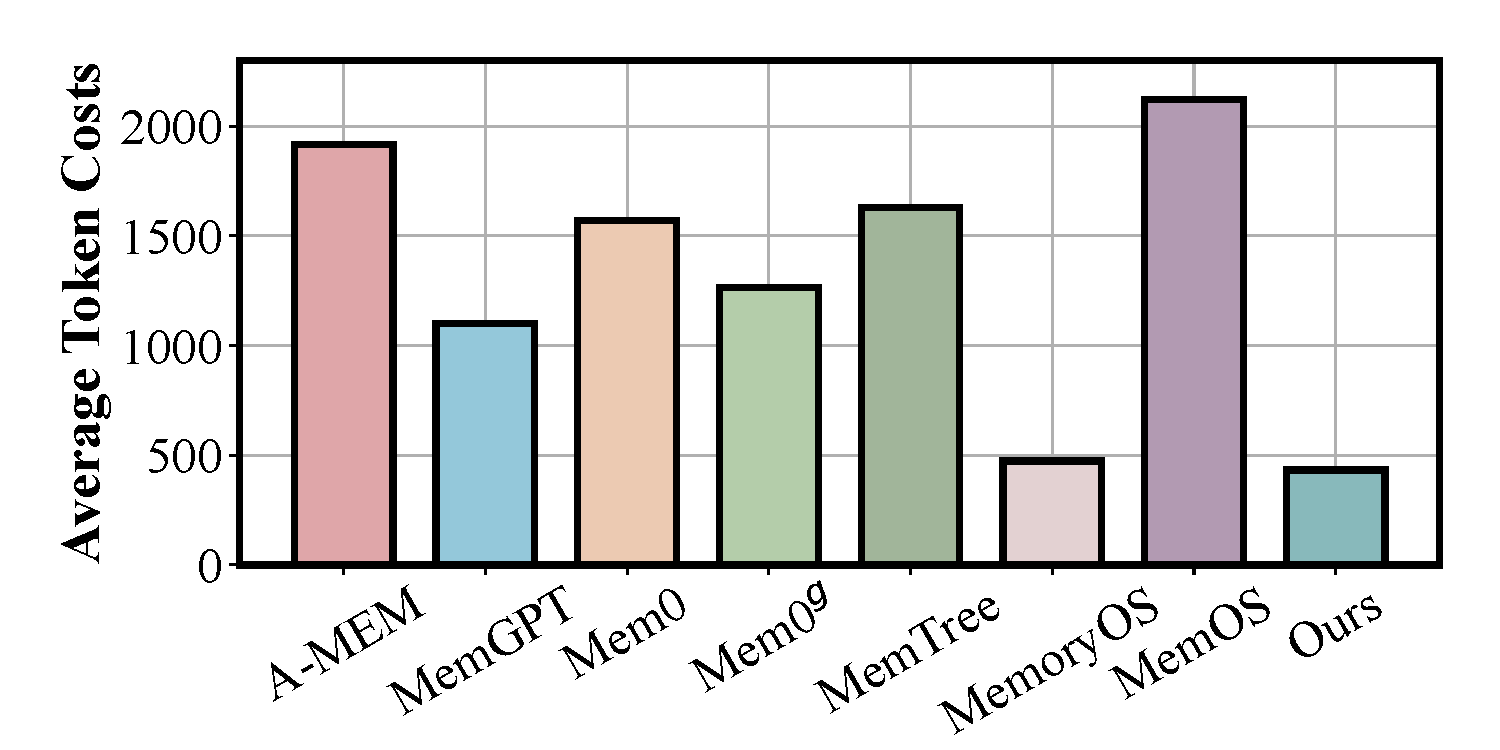
\includegraphics[width=0.97\linewidth]{figures/sotacost.pdf}
    \setlength{\abovecaptionskip}{0pt}
    \setlength{\belowcaptionskip}{5pt}
    \caption{Comparison of our newly designed method in terms of average token costs.}
    \label{fig:sota_cost}
\end{figure}








\begin{table*}[]
\centering
\caption{Comparison of our newly designed method on LOCOMO using Qwen2.5-7B/72B-Instruct (F1 Score).}
\label{tab:sota_loco}
\small
\begin{tabular}{l|l|r|r|r|r|r|r|r|r|r|r}
\toprule
\textbf{Category} & Size & \multicolumn{1}{c|}{\tt A-MEM} & \multicolumn{1}{c|}{\tt MemoryBank} & \multicolumn{1}{c|}{\tt MemGPT} & \multicolumn{1}{c|}{\tt Mem0} & \multicolumn{1}{c|}{\tt Mem0$^g$} & \multicolumn{1}{c|}{\tt Zep} & \multicolumn{1}{c|}{\tt MemTree} & \multicolumn{1}{c|}{\tt MemoryOS} & \multicolumn{1}{c|}{\tt MemOS} & \multicolumn{1}{c}{\tt Ours} \\
\midrule
\multirow{2}{*}{Single-Hop Retrieval} & 7B & 33.11 & 15.34 & 21.31 & 25.92 & 27.90 & \snd{40.42} & 33.36 & 33.14 & 39.55 & \fst{45.11} \\
& 72B & 42.24 & 24.54 & 28.78 & 32.83 & 29.58 & 42.46 & 38.73 & 43.56 & \snd{44.30} & \fst{48.01} \\
\midrule
\multirow{2}{*}{Multi-Hop Retrieval} & 7B & 25.38 & 16.63 & 18.92 & 19.43 & 21.14 & \snd{30.97} & 26.40 & 28.52 & \fst{34.04} & 30.01 \\
& 72B & 27.87 & 23.28 & 24.21 & 25.35 & 30.22 & 33.11 & 33.01 & 36.32 & \snd{36.67} & \fst{38.08} \\
\midrule
\multirow{2}{*}{Temporal Reasoning} & 7B & 14.69 & 11.57 & 17.37 & \snd{37.49} & 35.70 & 22.64 & 25.62 & 17.65 & \fst{37.55} & 32.23 \\
& 72B & 28.01 & 13.21 & 20.28 & 40.76 & 43.89 & 34.58 & 29.81 & 37.36 & \fst{49.59} & \snd{43.97} \\
\midrule
\multirow{2}{*}{Open-Domain Knowledge} & 7B & 14.69 & 16.09 & 11.14 & 16.93 & 18.67 & 21.79 & 20.67 & \snd{22.05} & \fst{22.55} & 18.92 \\
& 72B & 23.27 & 19.12 & 16.42 & 21.04 & 20.37 & 15.87 & 23.02 & 22.57 & \fst{24.88} & \snd{24.27} \\
\midrule
\multirow{2}{*}{Overall} & 7B & 26.71 & 14.84 & 19.42 & 26.58 & 27.71 & 33.82 & 29.68 & 28.34 & \snd{37.05} & \fst{38.03} \\
& 72B & 30.35 & 21.61 & 25.40 & 32.38 & 32.07 & 37.45 & 34.85 & 39.63 & \snd{42.79} & \fst{43.87} \\
\bottomrule
\end{tabular}
\end{table*}




\begin{tikzpicture}
\filldraw (0,0) -- (-0.15,0.08) -- (-0.15,-0.08) -- cycle ; 
\end{tikzpicture} 
\textbf{Exp.6. New SOTA algorithm.}
Based on the above analysis, we design a new memory framework that achieves state-of-the-art performance while maintaining low token overhead. Our approach integrates the tree-based organization of \texttt{MemTree} and \texttt{MemOS} with the hierarchical storage architecture of \texttt{MemoryOS}, categorizing memory into short-term, mid-term, and long-term tiers. Figure~\ref{fig:sota} illustrates the framework of our newly designed method, and the detailed workflow and algorithm are provided in Appendix~\ref{sec:app:ours}.

Table~\ref{tab:sota_lme} and Table~\ref{tab:sota_loco} report the performance metrics, and Figure~\ref{fig:sota_cost} compares the average token costs. 
Our method achieves the best overall performance on both benchmarks and delivers highly competitive results across all task categories, while maintaining a remarkably low computational overhead of fewer than 450 tokens per dialogue. 
Specifically, on LONGMEMEVAL, our method ranks first or second across all evaluated categories. Compared to the best-performing existing method, it achieves a relative F1 score improvement of 13.08\% on the Information Extraction-assistant task, and outperforms the strongest baseline by 5.17\% in the overall score. 
On LOCOMO, our method also achieves the best overall performance, surpassing the strong baseline {\tt MemOS}, and delivers consistently strong results across all categories, with particularly pronounced gains under the Qwen2.5-72B backbone. 
While baselines like {\tt MemOS} achieve higher scores on specific complex tasks (e.g., Multi-Hop Retrieval and Temporal Reasoning) by integrating multiple costly modules, our method strikes an optimal balance between performance and token efficiency, securing the best overall performance with a much more lightweight architecture.
Moreover, as shown in Table~\ref{tab:model}, our method remains competitive across a wide range of LLM backbones, demonstrating robust generalization.


\begin{figure}[t]
    \centering
    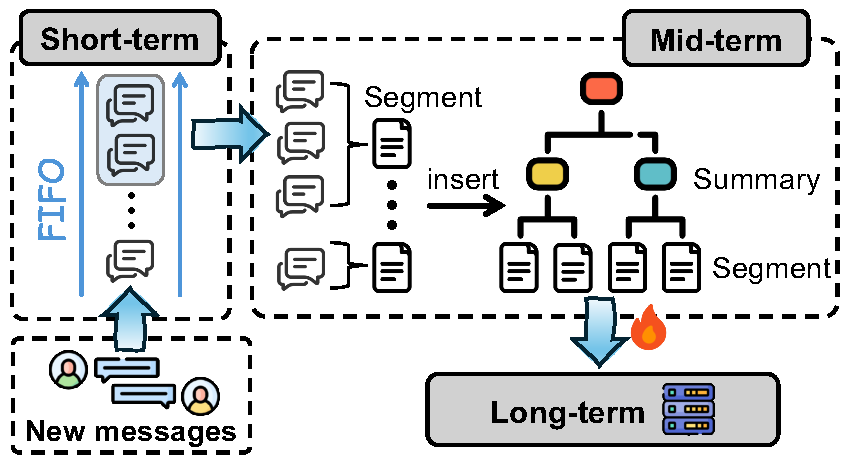
\includegraphics[width=0.97\linewidth]{figures/sota.pdf}
    \setlength{\abovecaptionskip}{3pt}
    \setlength{\belowcaptionskip}{1pt}
    \caption{The framework of our newly designed method.}
    \label{fig:sota}
\end{figure}
